\documentclass[10pt,A4paper]{article}
\usepackage[a4paper,
            inner=2.5cm,
            outer=3cm
            ]{geometry}

\usepackage[utf8]{inputenc}
\usepackage[a4paper,
            inner=2.5cm,
            outer=3cm
            ]{geometry}
            
\usepackage{graphicx}% Include figure files
%\usepackage{dcolumn}% Align table columns on decimal point
\usepackage{bm}% bold math
\usepackage{color}
%\usepackage[subnum]{cases}
\usepackage{hyperref}
\usepackage[backend=biber,
            sorting=none,
%            citestyle=numeric-comp,
%\            bibstyle=ieee, 
            style=numeric-comp,
            hyperref=true,
            maxnames=2,
            url=false,
            isbn=false,
            eprint=false,
            date=year,
            doi=false,
            giveninits=true
            ]{biblatex}
\addbibresource{references.bib}
\usepackage{xpatch}
\xpatchbibmacro{journal+issuetitle}{%
\usebibmacro{journal}%
\setunit*{\addspace}%
}{%
\usebibmacro{journal}%
\setunit*{\addcomma\space}%
}{}{}

\renewbibmacro*{name:andothers}{% Based on name:andothers from biblatex.def
  \ifboolexpr{
    test {\ifnumequal{\value{listcount}}{\value{liststop}}}
    and
    test \ifmorenames
  }
    {\ifnumgreater{\value{liststop}}{1}
       {\finalandcomma}
       {}%
     \andothersdelim\bibstring[\emph]{andothers}}
    {}}


%\DeclareFieldFormat[article]{title}{#1}
\DeclareFieldFormat[article]{volume}{\textbf{#1}}
%\DeclareFieldFormat[book]{volume}{\textbf{#1}}

\renewcommand\newunitpunct{\addcomma\space}
\DefineBibliographyStrings{english}{%
page = {},
pages = {},
}

\renewbibmacro{in:}{\addcomma\addspace}

\renewbibmacro*{volume+number+eid}{%
\isdot
\printfield{volume}%
\setunit*{\addcomma\addspace}%
\iffieldundef{number}{}{%
\printtext{no\adddot\addnbthinspace}%
}%
\printfield{number}%
\setunit{\addcomma\space}%
\printfield{eid}}


\setlength{\tabcolsep}{1.3pt}
\usepackage{bm}
\usepackage{amsmath}
\usepackage{amssymb}
\usepackage{mathtools}
\usepackage{mathrsfs}
\usepackage[T1]{fontenc}
\usepackage{diagbox}
\usepackage{here}
\usepackage[dvipsnames]{xcolor}
\usepackage{lipsum}
\usepackage{multirow}
\usepackage{ctable} % for \specialrule command
\usepackage{array,booktabs}
\newcolumntype{M}[1]{>{\centering\arraybackslash}m{#1}}
\usepackage{subcaption}
\usepackage{float}
\restylefloat{table}
\numberwithin{equation}{section}

\newcommand{\mbP}{\textbf{P: }}
\newcommand{\mbC}{\textbf{C: }}
\newcommand{\mbx}{\mathbf{x}}
\newcommand{\mbm}{\mathbf{m}}
\newcommand{\mbp}{\mathbf{p}}
\newcommand{\mbu}{\mathbf{u}}
\newcommand{\mbF}{\mathbf{F}}
\newcommand{\mbH}{\mathbf{H}}
\newcommand{\cmtb}[1]{\textcolor{blue} {#1}}
\newcommand{\cmt}[1]{\textcolor{red} {[#1]}}

\title{Pool Model Paper}
\author{Polina Gaindrik}


\begin{document}
\maketitle

\tableofcontents

\newpage

\section{Introduction}

...

- See Papers.

- Different processes in bacterial communities. 
Differents states, lag-phase, growth, stationary state. What processes behind.
Activation/inhibition/waste production, resource competition, back-flow to lag-phase.

- About known models for Predictive Microbiology Modelling, e.g., Baranyi/Roberts

\section{Motivating Example}

...

\cmtb{Maybe add here motivations about bacteria states: So toy system where we can eliminate states (sum and get F(n1, n2)).
And describe it initially without states/1state. Get the difference.}

\cmtb{Maybe Example from Seminar by Jens? 2 species,  1 resource, 1 waste production.}

\section{General Mathemetical Formulation}
Consider the system conssisting of $N$ species in $M$ different states.
In the general representation the system can be described with the Ordinary Differential Equations (ODEs) using a non-linear function $\mbF$:
\begin{equation}
   \dot{\mbx} = \mbF(\mbx, \mbm, \mbp, \mbu),
   \label{eq:model_ODE}
\end{equation}
where  $\mbx \in \mathbb{R}^{N}  \otimes \mathbb{R}^{M}$ is a vector descibing bacterial count.
In a matrix form it can be written as
\begin{equation}
    \mbx = \begin{pmatrix}
        x^1_1  & \dots & x^1_M  \\
        \vdots &       & \vdots \\
        x^N_1  & \dots & x^N_M  \\
            \end{pmatrix}
    \label{eq:model_bact}
\end{equation}
with $x_{ij}$ describing the bacterial counts for species $i$ in state $j$.
$\mbu$ is the vector of different inputs of the model, e.g., temperature, pressure etc.
The vector $\mbm \in \mathbb{R}^{K}$ includes all variables corresponding to the microenvironment of the system which can be concentartion of the inhibitors or activators:
\begin{equation}
    \dot{\mbm} = \mbH (\mbx, \mbm, \mbp, \mbu, ...).
    \label{eq:model_microenv}
\end{equation}
Here function $\mbH$ is in general case also non-linear.

The advantage of the following formulation is its generality. 
Depending on the knowledge about system as well as the needed level of accuracy one can define arbitrary number of states $M$ and control the complexity of teh model.
Moreover, opposite to the already known Predictive Microbiology like Baranyi and Roberts one can easily change.

To calculate the bacterial count for one species $i$, we simply need to sum the tensor/vector $\mbx$ over all possible states:
\begin{equation}
    N_n = \sum_m \mbx_i^n.
\end{equation}
While the total bacterial count of all species of our system is
\begin{equation}
    N_t = \sum_j \sum_m \mbx_i^j.
\end{equation}
In the following section we demonstate the application of this approach for different toy models describing the processes within and between bacteria communities.

\newpage

\section{One Species Modelling}
\subsection{Three-Pool Model}

Consider for simplicity the system where only one bacteria species is present $N=1$.
The bacterial growth curves usually consists of different consecutive phases~\cite{buchanan_when_1997}.
At the beginning no increase in bacterial count is present and so-called lag-phase is observed.
This phenomenon appears due to adaptation of the microbial community, for example, to the new environmental conditions.
This so-called preparation to the exponential growth includes synthesys of the needed compounds, initiation of the transciption~\cite{rolfe_lag_2012} and poorly studied physiological and regulatory mechanisms~\cite{monod_growth_1949,}
\cmt{For example, in Baranyi and Roberts modelling of lag-phase ???(maybe add).}
After this, the succeeded in adaptation bacteria enter the exponential growth phase, where the process of cell division is directly happening \cmt{Add Ref}.
When the nutrition is exhausted by the growing bacteria, the stationary state of the growth curve occurres.
In this state the cultures accumulate waste products of metabolitic activity that leads to cell death of the bacteria.
At the same time dying cells release the nutritions for survivors to continue growing.
As a result the balance between the growing and dyuing processes leads to the constant with time bacterial count~\cite{navarro_llorens_stationary_2010}.
In the described simplified version of the real-life system three possible bacteria states are mentioned corresponding to which process is happeng: adaplation, growth or death.
Motivated by this we divide a bacterial population into three pools (states) (\textbf{Figure \ref{fig:SchematicRep}}): 
\begin{itemize}
\item $L(t)$: the fraction of the population in the lag phase
\item $G(t)$: the fraction of the population growing and dividing
\item $D(t)$: the fraction of the population undergoing cell death
\end{itemize}
Here the concentrations of the pools are components of our variable vector $\mbx (t) =\{L(t), G(t), D(t)\}$.

\begin{figure}[t]
    \begin{center}
    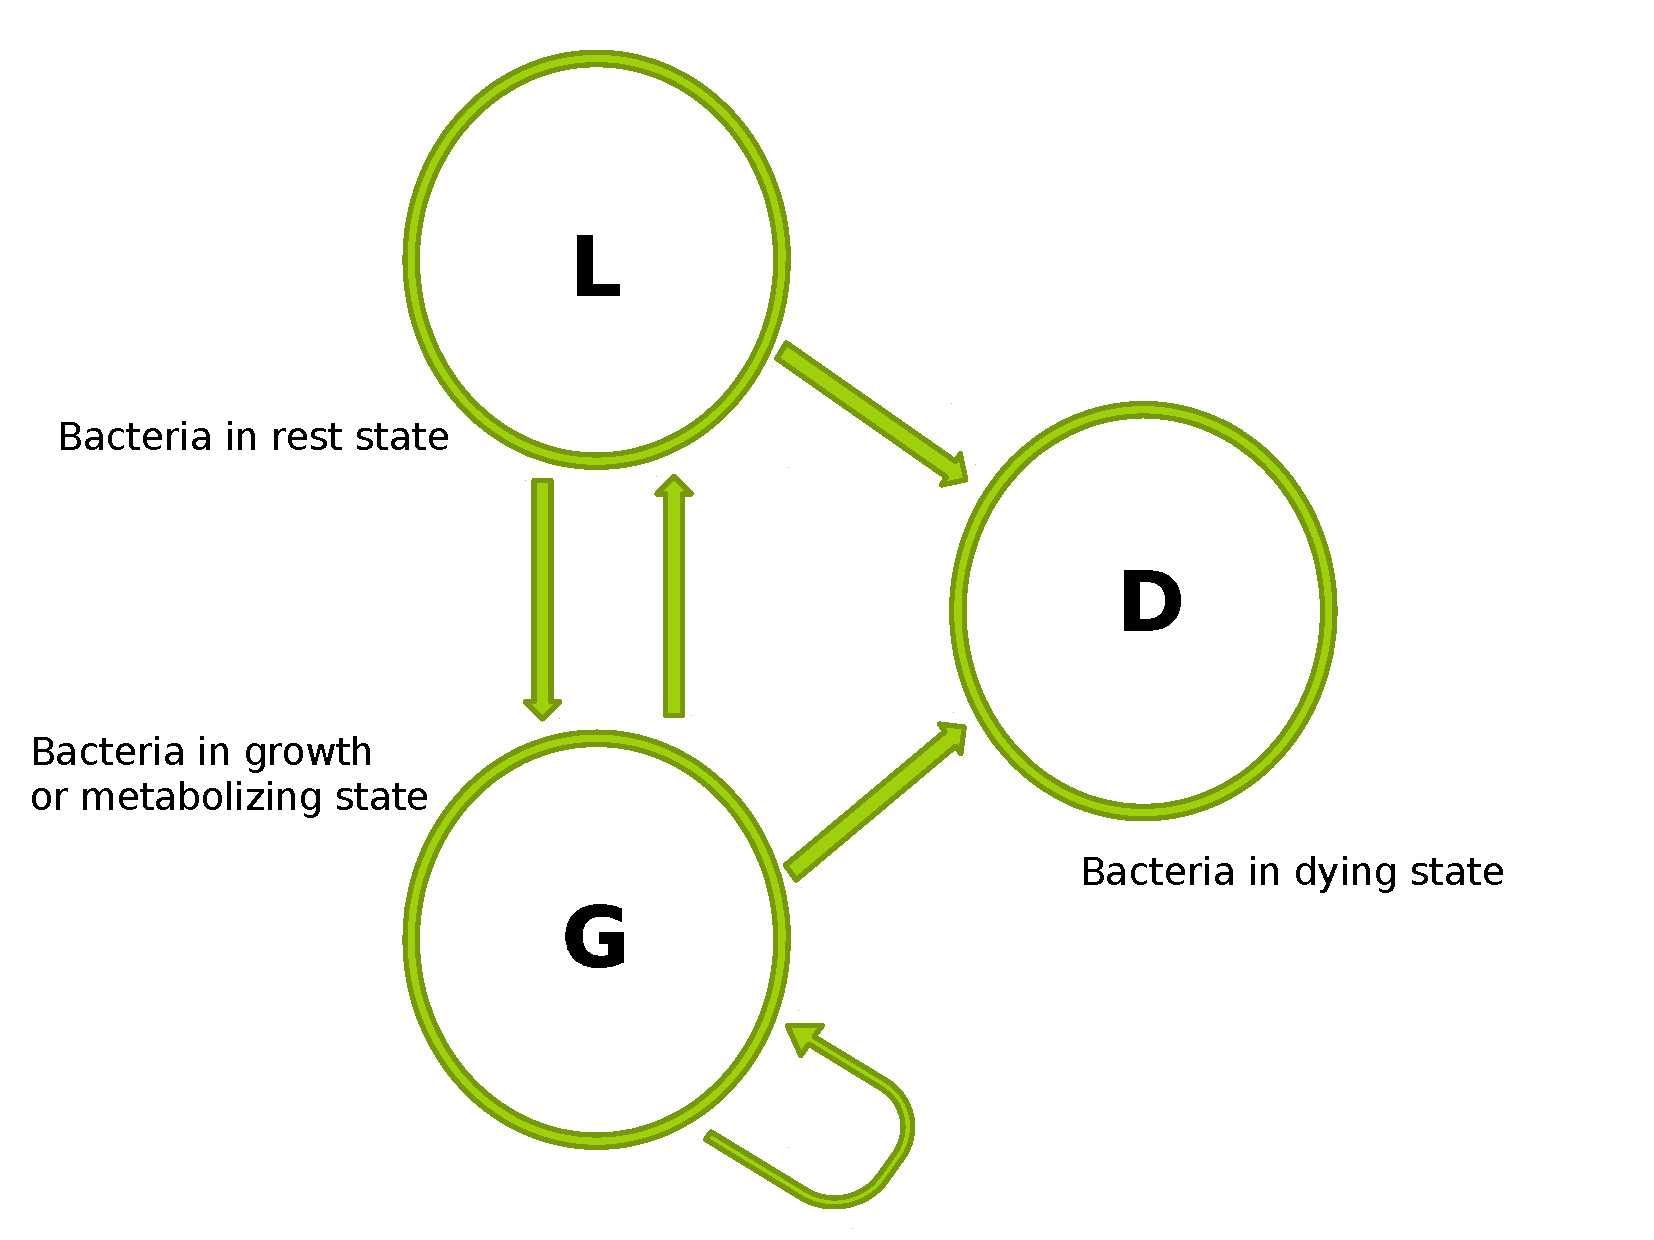
\includegraphics[width=0.7\textwidth]{Figures/TPM_fig.pdf}
    \caption{Schematic representation of exchange between three states or pools.}
    \label{fig:SchematicRep}
    \end{center}
    \end{figure}

To detremine the function $\mbF(\mbx, \mbm, \mbp, \mbu)$ consider the flows between different states.
The pools $G$ and $D$ are unidirectionally connected with the pool $L$. 
For now we assume for simplicity that there is no back flow between growth state $G$ and lag-state $L$. 
The suggested model can be cast in the following reactions:
\begin{eqnarray}
L &\stackrel{\lambda}{\longrightarrow} & G\\
L &\stackrel{\mu}{\longrightarrow} & D\\
G &\stackrel{\alpha}{\longrightarrow} & 2G\\
G &\stackrel{\mu'}{\longrightarrow} & D\\
D &\stackrel{\beta}{\longrightarrow} & \emptyset
\end{eqnarray}.

Then the ODEs describing such a model can be written as 
\begin{equation}
\begin{cases}
    \dot{L} = -(\mu + \lambda) L\\
    \dot{G} = \lambda L + \alpha G - \mu' G\\
    \dot{D} = \mu  L + \mu' G- \beta D  
\end{cases}.
\end{equation}

\cmt{Add plots ?? Or already after resource is added?}

\subsubsection{Resource Dependence}

Based on experimental observations, it was shown that the bacterial growth is strongly influenced by the limiting resource.
In the system where all needed nutritients are in excess except for one the total growth is linear to the conentration of this liminting nutritient~\cite{hibbing_bacterial_2010, monod_growth_1949}.
The control of the population density with respect to the available nutritions is implemented using cell communication process called quorum sensing. 
Using release of the extracellular signalling molecules (autoinducers) it is possible to synchronize the gene expression of the whole group~\cite{ng_bacterial_2009}.

We would not dive into the processes of quorum sensing and try to keep it as simple as possible.
According to this, we aim to include a resource pool which is used by the growing bacteria using the second order kinetic reaction:
\begin{equation}
    G + R_0  \stackrel{\alpha_0}{\longrightarrow} 2G.
\end{equation}

Note that the pools $L$, $G$ and $D$ represent number of bacteria (or number of bacteria per unit area/volume) while $R_0$ represents an abstract resource pool. 
Let say $G=N_B/V$ and $[G]=1/V$, where $N_B$ is number of bacteria and $V$ is the volume. 
Then $R_0=N_R/V$ and $[R_0]=1/V$, where $N_R$ is the number of resource molecules (or any appropriate unit, e.g., mol). 
Then $[\alpha_0]=V/s$, $[N_t]=1/V$, and $[\alpha]=1/s$. 
For homogeneous densities it is equivalent to consider the total amount, i.e., multiplying $L$ and $G$ by the volume. 
In this case $[L]=[G]=[N_t]=1$.
For simplicity we rather make a transition to the dimensionless constant $\alpha:=\alpha_0 N_t$ and diminsioneless resource pool $R(t) = R_0 / N_t$ ($0 \leqslant R \leqslant 1$).
Here the full capacity of the resource pool $N_t$ was used as a scaling constant.
Then the growth term can be simply written as $\alpha G R$, and the microenvironment of the system introduced by \ref{eq:model_microenv} is defined by ODE:
\begin{equation}
\dot{R} = -\frac{\alpha}{N_t} R G
\end{equation}

Explointing that limitation of the resource pool also limits the total becterial count of the system  we find:
\begin{equation}
    R = 1 - \frac{L+G+D}{N_t}
\end{equation}
And, hence, the full system can be written as
\begin{equation}
    \begin{cases}
        \dot{L} = -(\mu + \lambda) L\\
        \dot{G} = \lambda L + \alpha G\left(1-\frac{L+G+D}{N_t}\right)-\mu' G\\
        \dot{D} = \mu  L + \mu' G- \beta D  
    \end{cases}.
\end{equation}



\cmt{Plots / results}

\subsubsection{Lag-time Estimation (??)}

Note that one could further simplify this model to a two pool or state model by omitting the pool $D$ and removing cells with rate $\beta$ directly from pool $L$. 
The relevant question here is whether cells in the pool $D$ still contribute to the limitation of the resources by, e.g., occupying space or consuming important nutrients. 
If yes, the three pool model would be advantageous, if not the two pool model is sufficient with the advantages of having one parameter less.\\

The dynamics of the three pool model can be captures by the coupled system of ordinary differential equations (the two pool model can be achieved by setting $D\equiv 0$ and replacing $\mu$ with $\beta$):
to be solved with the initial conditions $L(0)=n_0$, $G(0)=0$, and $D(0)=0$, where $n_0$ is the initial bacterial population. 
$N_t$ denotes the maximal size of the total bacterial population due to environmental limitations (\textbf{Figure \ref{GrowthDip}}). 
For $\mu'=0$ the equations for $L$ and $D$ can be readily integrated resulting in:
\begin{eqnarray}
L(t) &=& n_0 e^{-(\mu+\lambda)t}\\
D(t) &=& n_0 \mu e^{-\beta t}\frac{1-e^{-(\mu+\lambda-\beta)t}}{\mu+\lambda-\beta}.
\end{eqnarray}
For constant parameters $\mu$, $\lambda$, and $\beta$ the integrals for $L$ and $D$ can be put into the differential equation for $G$. 
However, for time dependent parameters, e.g. for a dependence on a non-static, dynamic temperature, it appears to be not advantageous to use the analytical results for $L$ and $D$ and work instead with all three equations for $L$, $G$, and $D$. 
It is interesting to see what type of equations result for the total bacterial population $n=L+G+D$:
\begin{eqnarray}
\dot{G} &=& \lambda L + \alpha G\left(1-\frac{n}{N_t}\right)\\
\dot{n} &=& - \beta D + \alpha G\left(1-\frac{n}{N_t}\right). 
\end{eqnarray}
with the initial conditions $G(0)=0$ and $n(0)=n_0$. 
These equations have a clear interpretation, are derived from simple principles, and are different from the popular Barayni-Roberts and modified-Gompertz models. 
A notable difference is that the growth rate $\alpha$ is time independent. 
For the functions $L$ and $D$ it holds: $\lim_{t\to\infty} L(t) = \lim_{t\to\infty} D(t) = 0$. 
It follows immediately that $\lim_{t\to\infty} G(t) = N_t$. 
The equation exhibit a lag phase and an initial drop due to cell death. 
To find a substantial initial drop one needs $\beta \mu \gg \alpha \lambda$. 
The lag time $t_L$ can be approximated by the time at which half of the initial population is in the growth phase, i.e., $n_0=2G(t_L)$. 
Assuming $L\ll N_t$ we can ignore the non-linear term in the equation for $G$, which gives rise to:
\begin{eqnarray}
1&=& 2\int_0^{t_L} \lambda L(t)e^{\alpha(t_L-t)}dt\\
1  &=& 2\lambda e^{\alpha t_L}\frac{1-e^{-(\mu+\lambda+\alpha)t_L}}{\mu+\lambda+\alpha}.
\end{eqnarray}
For $\alpha > \mu+\lambda$ $t_L$ can be approximated by:
\begin{eqnarray}
t_L &\approx& -\frac{1}{\alpha}\ln\left(\frac{2\lambda}{\mu+\lambda+\alpha}\right).
\end{eqnarray}
The lag time $t_L$ diverges very slowly, logarithmically with $\lambda\to 0$.

\cmt{Add/make plots to the model 3 pool/ 2 pool.}

\cmt{Add limitation due to resource}

\subsection{Resource-dependent lag-phase}

Another way to encorporate the resource dependence is to assume that the bacteria only leave the lag-phase if there are nutrients, i.e., resources. 
Otherwise they stay in the lag-phase.
Then using the model consisted of two bacteria states $L$ and $G$ we can define the system as
\begin{eqnarray}
\dot{L} &=& - \lambda R L\\
\dot{G} &=& \lambda R L +\alpha R G\\
\dot{R} &=&-\frac{\alpha}{N_t} R G.
\end{eqnarray}


Turning back to the equations above we can state: $L+G+N_tR=N_t$. For $t=0$ we have $n_0+N_tR_0=N_t$ (given $L_0=n_0$ and $G_0=0$) and from this: $N_tR_0=N_t-n_0$. Using this we eliminate $R$ and arrive at: 
\begin{eqnarray}
\dot{L} &=& - \lambda \left(1-\frac{L+G}{N_t}\right)L\\
\dot{G} &=& \lambda \left(1-\frac{L+G}{N_t}\right)L +\alpha \left(1-\frac{L+G}{N_t}\right) G
\end{eqnarray}
The steady state is $L_s+G_s=N_t$. However, it depends on the initial conditions and the parameters what $L_s$ and $G_s$ are. There is no way to determine $L_s$ and $G_s$ besides solving the dynamical equations, i.e., the steady state cannot be determined directly by solving a set of algebraic equations. To see this we determine the nullclines: the first nullcline is $G=N_t-L$ and the second is $G=N_t-L$, i.e., the nullclines coincides. Every point on the line $G=N_t-L$ is a fixed point. 
This can be seen in Fig. \ref{Phaseplot}. 
For $\lambda\ll \alpha$ the lag-pool is not emptied before all resources are consumed. As a consequence the lag-pool is non-zero in steady-state. 
In contrast, for $\lambda\gg \alpha$ the lag-pool is depleted before the resources are consumed, i.e., the lag-pool is zero in steady state.

The fraction $G$ of the exponentially growing cells will go to steady state due to limitations in resources. 
$\lambda$ is the rate by which cells go from the lag phase to the growth phase; $\mu$ is the rate by which cells go from the lag phase to the state in which they die; $\alpha$ is the growth rate of the healthy population; $\beta$ is the rate by which the cells are removed from the $D$ pool. 

\cmt{Plots / results}

\subsection{Back flow from G to L}

Due to the life in rather unfavourable conditions bacteria developed different surviving mechanisms, one of which is adapting their metabolism and transitioning into dormant state.
By defeinition dormancy in bacteria is a reversible state where cell continue living with low metabolic activity while the cell division stops~\cite{kaprelyants_dormancy_1993}. 
This survival strategy can appear in response to different external stresses, e.g., nutritient deficiency, temperature stress or extreme fluctuations of environment parameters.
And after "difficult times" bacteria, also called viable but non-culturable(VBNC), can continue cell division~\cite{kell_viability_1998}.
The models including transition of bacteria to the dormant state were proposed and studied by Bär \etal~\cite{bar_modelling_2002} and Jones and Lennon~\cite{jones_dormancy_2010}.

\cmt{So now is it better to use flow to dormancy instead?}


We explore now the idea that under certain conditions, as sudden change in the environment, part of the population $G$ will enter a lag-phase, i.e., there is a back-flow from $G$ to $L$. 
\begin{eqnarray}
L &\stackrel{\lambda}{\longrightarrow} & G\\
L &\stackrel{\mu}{\longrightarrow} & D\\
G &\stackrel{\alpha}{\longrightarrow} & 2G\\
G &\stackrel{\gamma(t)}{\longrightarrow} & L\\
D &\stackrel{\beta}{\longrightarrow} & \emptyset
\end{eqnarray}
The rate $\gamma(t)$ depends on the rate of change of the environment. Stronger and quicker changes will lead to a higher rate $\gamma$. 
Let the change in the environment be in temperature $T$ (\textbf{Figure \ref{default}}).

\subsubsection{Maxwell type of stress - strain relation}

One of the reasons of the dormant state appearence can be also the temperature shift~\cite{oliver_viable_1995}.

We propose a kind of visco-elastic Maxwell type of stress-strain relation and write down the ordinary differential equation for $\gamma$ to be:
\begin{eqnarray}
\dot{\gamma} &=& \Gamma \left |\dot{T}\right |-\delta \gamma.
\end{eqnarray}
We assumed that the direction of the temperature change does not matter, i.e., a change from $T=2$ to $T=12$ has the same effect as a change from $T=14$ to $T=4$. 
$\Gamma$ is a scaling factor and $\delta$ is the relaxation time for the temperature disturbance. 
Integration of this equation yields (with $\gamma(0)=0$):
\begin{eqnarray}
\gamma(t) &=& \Gamma \int_0^t \left |\dot{T}(t^{\prime})\right |e^{-\delta (t-t^{\prime})}dt^{\prime}.
\end{eqnarray}
After some manipulation of this equation we find:
\begin{eqnarray}
\gamma(t) &=& \Gamma\delta\left |\left[T[t]-T[0]e^{-\delta t}-\delta \int_0^t T(t^{\prime})e^{-\delta (t-t^{\prime})}dt^{\prime}\right]\right |.
\end{eqnarray}
This representation of the rate $\gamma(t)$ has the advantage that it only involves $T(t)$ and does not require the calculation of the derivative of $T$. 
If $T$ exhibits $n$ temperature jumps, one finds:
\begin{eqnarray}
\gamma(t) &=& \Gamma\sum_{i=1}^n \left |\Delta T_i \right |\theta(t-t_i)e^{-\delta(t-t_i)}.
\end{eqnarray}

The ordinary differential equations for the pool model with environmental-shock based back-flow read:
\begin{eqnarray}
\dot{L} &=&\gamma(t) G - (\mu + \lambda) L\\
\dot{G} &=& \lambda L -\gamma(t) G + \alpha G\left(1-\frac{L+G+D}{N_t}\right)\\
\dot{D} &=& \mu  L - \beta D
\end{eqnarray}

-  \cmt{Ref to temperature jumps effect. Plots / results.}


\newpage

\section{Interaction between species}

As it was mentioned above, bacteria usually coexist in large multispecies interacting communities whose growth is vastly determined by the developed survival mechanisms.
These survival mechanisms mostly aim to secure as much available nutrition which lead to competitive strategies or, if it is advantageous, cooperative ones~\cite{hibbing_bacterial_2010, stubbendieck_bacterial_2016}.
Further we show that the TPM can be readily extended to the systems with more than one bacteria an take describe more complex relationships between species. 


\subsection{Resource Competition}

One on the ways to descibe competition between bacteria populations is as a function of limiting resources ratio~\cite{tilman_resource_1977, smith_effects_2002}.
To descibe such a situation we consider for simplicity only one common limiting resource pool. 
The simplest pool model for bacterial species $A$ and $B$ encompassing lag-phases, growth-phases and a common resource pool is given by (no back-flow to the lag-pool):

\begin{eqnarray}
\label{Model_Comp1}
\dot{L}_A &=& - \lambda_A R L_A\\
\dot{L}_B &=& - \lambda_B R L_B \\
\dot{G}_A &=& \lambda_A R L_A +\alpha_A R G_A\\
\label{Model_Comp4}
\dot{G}_B &=& \lambda_B R L_B +\alpha_B R G_B\\
\dot{R} &=&-\frac{\alpha_A}{N_t} R G_A-\frac{\alpha_B}{N_t} R G_B
\end{eqnarray}
We again rescaled the resource pool with $N_t$ and find
\begin{eqnarray}
\label{Resource}
R &=&1-\frac{L_A+G_A+L_B+G_B}{N_t}\\
R_0&=&1-\frac{n_A+n_B}{N_t}. 
\end{eqnarray}
Inserting Eq. \ref{Resource} into Eqs. \ref{Model_Comp1} - \ref{Model_Comp4} yields:
\begin{eqnarray*}
\dot{L}_A &=& - \lambda_A  L_A + \frac{\lambda_A}{N_t}\left(L_A+G_A+L_B+G_B\right )L_A\\
\dot{L}_B &=& - \lambda_B L_B + \frac{\lambda_B}{N_t}\left(L_A+G_A+L_B+G_B\right )L_B \\
\dot{G}_A &=&  \lambda_A  L_A - \frac{\lambda_A}{N_t}\left(L_A+G_A+L_B+G_B\right )L_A +\alpha_A G_A - \frac{\alpha_A}{N_t}\left(L_A+G_A+L_B+G_B\right )G_A\\
\dot{G}_B &=& \lambda_B L_B - \frac{\lambda_B}{N_t}\left(L_A+G_A+L_B+G_B\right )L_B  +\alpha_B G_B -\frac{\alpha_B}{N_t}\left(L_A+G_A+L_B+G_B\right )G_B
\end{eqnarray*}

which has the structure of a generalised Lotka-Volterra system (gLV). \cmt{Add reference about Lotka-Volterra. Compare with different states LV.}
In order to better see this, we set $L_A=L_B=0$: 
\begin{eqnarray}
\label{Comp_Model}
\dot{G}_A &=& \alpha_A G_A\left(1 - \frac{G_A}{N_t}\right ) - \frac{\alpha_A}{N_t}G_AG_B\\
\dot{G}_B &=& \alpha_B G_B\left(1-\frac{G_B}{N_t}\right ) -\frac{\alpha_B}{N_t}G_AG_B. 
\label{eq:LV_simple}
\end{eqnarray} 

Equations (\ref{eq:LV_simple}) are basically competitive Lotka-Volterra equations that are widely used in ecological studies and show the principle of competive excursion.
That principle claims that two species in competition for the same resource cannot coexist~\cite{wangersky_lotka-volterra_1978}. 
In previous studies it was shown that gLV equations can be sucessfully applied to predict the microbial community dynamics, determine different types of the pairwise interspecies interactions~\cite{dedrick_when_2023, stein_ecological_2013, venturelli_deciphering_2018, hoffmann_power_2007}.
In food studies the gLV was applied by Mounier \etal~\cite{mounier_microbial_2008} to study interactions of 6 bacteria species  with yeast omissin in cheese.

For $N_t\gg\alpha_{A/B}$ the equations decouple. 
The null-clines of the system given by Eqs. \ref{Model_Comp1} - \ref{Model_Comp4} coincide and are given by $N_t=L_A+G_A+L_B+G_B$. 
If $\lambda_{A/B}>\alpha_{A/B}$ the lag-pools are completely depleted before the depletion of the resource pool stops the dynamics. 
To simplify the investigation of the systems dynamics we therefore ignore the $L_A$ and $L_B$ dimension and only consider the dynamics on the centre-manifold given by the $G_A\times G_B$ plane. 
The corresponding phase-plot is shown in Fig. \ref{Competition}. 
The advantage in using the pool model in contrast to using Lotka-Volterra directly is that all parameters have a clear meaning and consistent parameter relations arrive naturally. 
And a species can have more than one internal state. 
However, it is instructive to rewrite the system by setting $x_1\equiv G_A$, $x_2\equiv G_B$, and $\mathbf{x}=(x_1,x_2)^T$:

\begin{eqnarray}
\dot{\mathbf{x}}&=&A\mathbf{x}+\frac{1}{2}\mathbf{x}B\mathbf{x}\\
A&=&
\begin{bmatrix}
\alpha_A&0\\
0 &\alpha_B
\end{bmatrix}\\
B&=&
\frac{-2}{N_t}\begin{bmatrix}
\alpha_A&\alpha_A\\
\alpha_B &\alpha_B
\end{bmatrix}
\end{eqnarray}

The pool model, in contrast to the classical Lotka-Volterra approach, allows for far more flexibility. 
Non-linear functional responses can be introduced without any problem (see how section \ref{Gen_Lot_Vol} for an extended discussion).

\cmt{Plots / results}

\cmtb{Look papers on modelling of the LV in bacterial communities. Did anyone do the same as we??}

\subsection{Interspecies Competition}

However, except the inhibition due to resource competition, bacteria developed differnt others active competition mechanisms.
One of the examples of such mechanisms is a production of the antimicrobial compounds, which can be also called antibiotics or inhibitors.

\cmt{Read how this antibiotics affect the system. Which eq form to use?}

\cmt{\cite{lenski_coexistence_1986}: Modelling of the 2 sp. system with 1resource and 1 inhibitor.}

Now extend our model where bacteria not only consume nutritions from resource pool $R$ but one of the species also actively produce the inhibiting compounds $I$. 
It is the accumulation of the bacteria waste which is responsible for the spoilage of food products. 
In order to take this into account we add an equation for the waste production:
\begin{eqnarray}
\dot{L} &=& - \lambda_f R L + \mathcal{B}(R)G\\
\dot{G} &=& \lambda_f R L +\alpha R G-\mathcal{B}(R)G\\
\dot{R} &=&-\frac{\alpha}{N_t} R G\\
\dot{I} &=& \mathcal{F}(R,G).
\end{eqnarray}
The function $\mathcal{F}$ denotes the model for the antibiotic production rate. 
We shall discuss two possible models:
\begin{eqnarray}
\mathcal{F}_1(R,G)&=&\kappa\alpha R G=-\kappa N_t\dot{R}\\
\mathcal{F}_2(R,G)&=&\kappa G
\end{eqnarray}
Model $\mathcal{F}_1$ results in waste accumulation in steady state $I_1^s=\lim_{t\to\infty}I_1(t)=\kappa(N_t-n_0)$. 
To see this we note $\dot{I}_1=\kappa(\dot{L}+\dot{G})$, which yields: $I_1(t)=\kappa(L(t)+G(t)-n_0)$ where we used $I_1(0)=G(0)=0$, $L(0)=n_0$. 
This model assumes that inhibitor is only produced when the bacteria grow and divide. \\

Model $\mathcal{F}_2$ results in $I_2(t)=\kappa\int_{t_0}^tG(t')dt'$. 
As long as $G>0$ inhibitor is produced, no matter whether the amount of bacteria is still growing. 
The amount of inhibitor depends therefore on the back-flow model employed, which can be seen in Fig. \ref{Waste}. 

\cmt{Look is this inhibition the same as waste production. Or change it.}


The simplest way to introduce inhibition of species A by species B is via a growth rate of species A depending on the abundance of species B. 
For sake of simplicity we ignore the lag pool and write for a mutual inhibition:
\begin{eqnarray}
\dot{G}_A &=& \mathcal{B}_A(G_B)G_A\left(1 - \frac{G_A+G_B}{N_t}\right )\\
\dot{G}_B &=& \mathcal{B}_B(G_A) G_B\left(1-\frac{G_A+G_B}{N_t}\right ). 
\end{eqnarray}
The function $\mathcal{B}_{A/B}$ captures the inhibiting effects in an effective way. 
It is straight forward to make the mechanism of inhibition more explicit by, e.g., introducing a waste pool. 
One possible choice for $\mathcal{B}$ is: 
\begin{eqnarray}
\mathcal{B}(G)&=&\frac{\alpha}{1+KG}. 
\end{eqnarray}
This corresponds to the case $W\sim G$, where $W$ is the waste (or whatever one chooses to call it) of species A affecting species B. 
If the waste accumulates one needs to replace $G$ by $\int G dt$. Keeping it simple yields:
\begin{eqnarray}
\dot{G}_A &=& \frac{\alpha_A G_A}{1+K_BG_B}\left(1 - \frac{G_A+G_B}{N_t}\right )\\
\dot{G}_B &=& \frac{\alpha_B G_B}{1+K_AG_A}\left(1-\frac{G_A+G_B}{N_t}\right ). 
\end{eqnarray}
One can distinguish two limiting cases: {\it i}) $K_{A/B}\ll N_t$ and {\it ii}) $K_{A/B}\gg N_t$. 
In the first case the inhibition is of minor importance and could be ignored. 
In the latter case one can simplify the equations, given $n_A$ and $n_B$ are non-zero:
\begin{eqnarray}
\label{Mut_Inhib}
\dot{G}_A &=&\tilde{\alpha}_A\frac{G_A}{G_B}\left(1 - G_A-G_B\right )\\
\dot{G}_B &=& \tilde{\alpha}_B\frac{G_B}{G_A}\left(1-G_A-G_B\right ). 
\end{eqnarray}
We introduced the rescaled growth rates $\tilde{\alpha}_A=\alpha_A/(N_tK_B)$ and $\tilde{\alpha}_B=\alpha_B/(N_tK_A)$. Note that $[\tilde{\alpha}]=\mathrm{s}^{-1}$. Rescaling time with $\tilde{\alpha}_A$ and defining the dimensionless parameter 
\begin{eqnarray}
\psi&=&\tilde{\alpha}_B/\tilde{\alpha}_A\\
\psi&=&\frac{K_B\alpha_B}{K_A\alpha_A}
\end{eqnarray}
results in: 
\begin{eqnarray}
\dot{G}_A &=&\frac{G_A}{G_B}\left(1 - G_A-G_B\right )\\
\dot{G}_B &=&\psi\frac{G_B}{G_A}\left(1-G_A-G_B\right ). 
\end{eqnarray}
We can separate three cases: 
\begin{eqnarray}
\psi&>&1:\quad\text{Species B growth faster and/or inhibits A stronger}\\
\psi&=&1:\quad\text{A and B are equivalent}\\
\psi&<&1:\quad\text{Species A growth faster and/or inhibits B stronger}
\end{eqnarray}

\subsection{Interspecies Cooperation}

On the other hand, one can also observe some cooperative behaviours between species in case when it facilitates the competition with others.
Quite often it happens between the species that are close relatives or clonal populations and such process is called kin selection \cite{west_social_2007}.
Sometimes neighbours, so-called 'social cheaters', can benefit from a certain behaviour without expressing it by itself \cite{rainey_evolution_2003}.

\cmt{\cite{rocha_base_2002}: Symbiosis host/bacteria. bacterial genomes suffering reductive evolution due to this. 
Maybe it's connected with 'social cheaters'?}

The benefit, or mutual activation, of the two species from the presence of the other can be simply introduced by mathematical functions. 
For sake of clarity we omit again the lag pool and write:
\begin{eqnarray}
\dot{G}_A &=& \mathcal{B}_A(W_B,R)G_A\\
\dot{G}_B &=& \mathcal{B}_B(W_A,R)G_B\\
\dot{R} &=&-\mathcal{B}_A(W_B,R)G_A-\mathcal{B}_B(W_A,R)G_B\\
\dot{W}_A &=& \mathcal{F}_A(R,G_A)\\
\dot{W}_B &=& \mathcal{F}_B(R,G_B).
\end{eqnarray}
$W_A$ and $W_B$ denote the substance produced by species A and B, respectively. 
The functions $\mathcal{B}_A(W_B,R)$ and $\mathcal{B}_B(W_A,R)$ capture the resource dependent growth. 
Setting $\mathcal{B}_A(W_B,R)=\alpha_A W_BR$, $\mathcal{B}_B(W_A,R)=\alpha_B W_AR$, $\mathcal{F}_A(R,G_A)=\kappa_A RG_A$, $\mathcal{F}_B(R,G_B)=\kappa_B RG_B$, rescaling $G_A$, $G_B$, and $W_B$ with $N_t$, $W_A$ with $\kappa_A/\alpha_A$, time with $\alpha_AN_t^2$, defining $\phi=\kappa_A\alpha_B/(\alpha_A^2N_t)$, and $\psi=\kappa_B/(\alpha_A N_t)$ results in: 
\begin{eqnarray}
\dot{G}_A &=& W_BG_A\left(1 - G_A-G_B\right )\\
\dot{G}_B &=& \phi W_AG_B\left(1 - G_A-G_B\right )\\
\dot{W}_A &=& G_A\left(1 - G_A-G_B\right )\\
\dot{W}_B &=&\psi G_B\left(1 - G_A-G_B\right ).
\end{eqnarray}

\section{Spatial Limitations}

\cmtb{Maybe as motivation can be spatial competitive mechanisms as adhesion to survaces and motility. 
So how much including these effects will affect system.}

\cmt{\cite{htuson_bacteriasurface_2013}: Attachment of bacteria to surfaces. (One of the mechanisms to stick to the areas with nutritients)}


\cmtb{We can take some toy model (e.g the one from group seminar) and do agent-based simulation. (add spatial component)
Then from this simulation we sum bacteria and get growth curves.
And using our model equations we get also growth curves.
And find prob diffusion coef, maybe rates where model works fine.
For sim maybe we will need to name specific bacteria species. (maybe nicer)}

\section{Conclusion}

\newpage
\printbibliography

\end{document}